\chapter{Discussion} \label{sec:discussion}

This section contains the discusses the results summarized in the previous Section on a per TD item basis, with a coarser clustering following the defined RQs. Each technical debt item is described following the structure proposed by Li et al.\ \cite{mapping_study_td}. However, fields not applicable to the nature of this study are omitted.

Finally, since one of the required fields in this proposed structure is the interest amount that is the raison d'etre of RQ3, the explanation is provided together with the description of every TD item. Therefore, a separate section for that RQ is omitted.

\section{Research Question 1} \label{sec:disc-rq1}

    \subsection{DRY violations} \label{sec:res-dry-violations}

        DRY is an acronym that stands for Don't Repeat Yourself. Its essence is about that logic should be implemented once and only once and reused in different sections of the code-base when needed.

        The accretion of this TD item happens in two different circumstances. Firstly, when the code is poorly documented is harder for maintainers to know which primitives and functionalities are available, and the more extensive the code base, the more developer incur in this problem.

        The other source of DRY violations is the lack of tooling. In fact, developers and testers alike agree that not having a full-fledged IDE (Integrated Development Environment) causes these problems.

        In the Company, both causes are present with the lack of documentation being the predominant one. In fact, UFT provides an IDE that is considered inferior to other tools available for Source Code Development like Eclipse or IntelliJ IDEA. Therefore, part of this TD manifestations can be caused from this. However, the interviews revealed this to be more of a nuisance than a problem. On the other hand, the lack of documentation is perceived as a real problem: testers need to browse the source code to understand what a function does. Moreover, when asked how familiar they are with the functionalities provided by the common repository or other parts of the test code-base none of the interviewees provided an answer ascribable to a good knowledge.

        \phantomsection
        \label{sec:disc-rq3-dry}
        Moreover, the severity of this TD item is even greater if considered from a holistic point of view. In fact, duplicated logic inflates function complexity by requiring testers to reimplement such logic and the single responsibility violation, since if the logic is duplicated it means it can be extracted into a reusable entity that does that task.

        For these reasons, the author believes that this TD item perfectly matches the correspondent one in source code TD with no differences. Moreover, the interviewees perceive this problem as serious (4.5/5 on Likert's scale); roughly the same as expressed by Hunt and Thomas in \textit{The pragmatic programmer} \cite{thomas1999pragmatic}.


    	\begin{table}[!htbp]
		\centering
		\tabulinesep=1.2mm
		\begin{tabu} to \textwidth {|X|X[3]|}

			\hline
			\textbf{Field} & \textbf{Value} \\
			\hline

			ID & DRY Violations \\
			\hline

			Location & Logic of UI tests \\
			\hline

			Responsible & Tester developer \\
			\hline

			Type & Code Technical debt \\
			\hline

			Description & Repeating the same logic of code in at least two different sections of the code-base\\
			\hline

			%Date / Time & Not applicable \\
			%\hline

			%Principal & Non applicable \\
			%\hline

			Interest amount &  4.5/5 (Between High and Very on Likert's scale) \\
			\hline

			%Interest probability & Not applicable \\
			%\hline

			%Interest standard deviation & Not applicable \\
			%\hline

			Correlations with other TD items & Functions Complexity, God functions\\
			\hline

			%Name & Not applicable \\
			%\hline

			%Context & Not applicable \\
			%\hline

			Propagation rules & It is very likely that it accrues since flattening a deeply nested hierarchy of statements is error-prone and tedious.\\
			\hline

			Intentionality & Both intentional and non \\
			\hline

		\end{tabu}
		\label{tab:res-dry-violations}
		\caption[DRY violations specification]{DRY violations specification according to guidelines specified by \cite{mapping_study_td}.}
	\end{table}

	\subsection{Function complexity}


	The first TD item analyzed is Function Complexity as measured by the Cyclomatic Complexity metric described by McCabe \cite{cyclomatic_complexity}.

    This TD item accrues in the source code that contain the logic behind the UI tests. Specifically, within the functions that manipulate both the global state (e.g.\ the UI under test) and the data retrieved from it once an action occurs. A function, in the Software Engineering field, refers to a named section of the source code that perform a specific task and can use an input or solely rely on modification of the mentioned global state. The analysis performed in this study does not differentiate between those two variants since cyclomatic complexity applies to both. This metric captures how complex is the directed acyclic graph that links one statement to the other. Loops, IF-ELSE constructs, etc.\ inflate such complexity by spanning branches and loops that make harder to reason about the data flow.

    In the Company under study, there are people appointed as testers who are in charge of developing and maintaining such code base. These people are appointed as responsible since the test code health is under their responsibilities. Furthermore, the accretion of this TD item is also intentional, since it is possible to distinguish between a plain, easy to follow function and an intricate one. Moreover, by their admission, once the test code is deployed and effectively enters the testing pipeline, it becomes harder to remedy and refactor. In fact, \textit{"even if the code is messy refactoring it is hard because many functions start using the code, ..., and fixing it always breaks something else or introduce errors ..." }. This could explain the crescent trends recognizable in Figures \ref{fig:avg-complexity-together}. In fact, despite active efforts (e.g.\ the drop in complexity in series A1 noticeable after a refactoring effort), the average complexity increases revision after revision with few exceptions.

    \begin{figure}[!htbp]
    	\centering
    	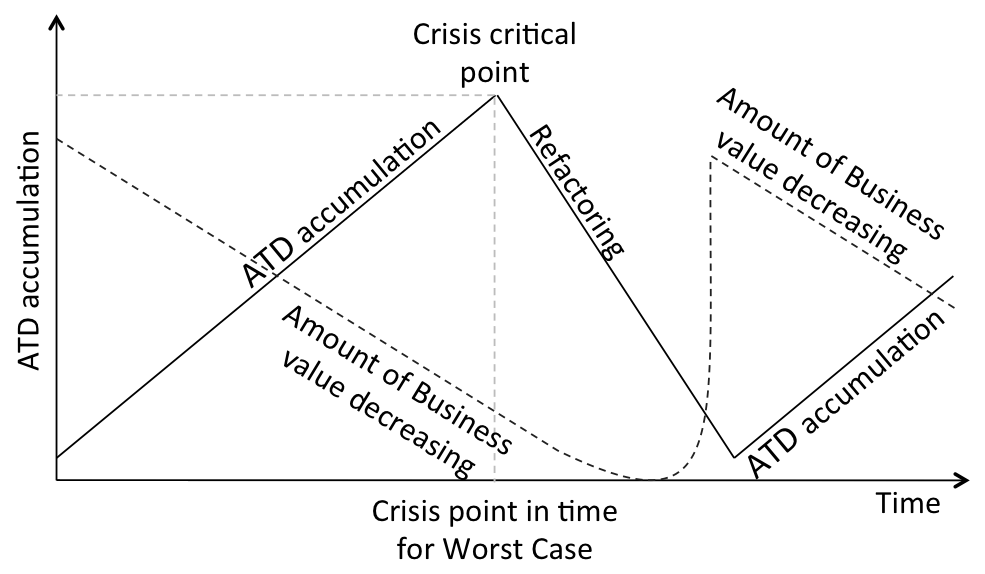
\includegraphics[width=\textwidth]{figure/discussion/martini-model.png}
    	\caption{Martini et al. \cite{martini2014architecture} model with Crisis point followed by a considerable refactoring.}
    	\label{fig:antonio-model}
		\end{figure}

    For all these reasons, the author of this study believes that the available knowledge on Function Complexity related to Technical Debt is widely applicable in the realm of UI testing, with little differences. Most notably, these differences are about which role the code base has (e.g.\ regression tests or smoke tests) and the threshold above which a function is considered too complex.


    \phantomsection \label{sec:disc-rq3-function-complexity}
    The first item is necessary since smoke tests are, by nature, shallow and hence less impacted by changes in the product. Therefore, the interest paid in such tests is low. On the opposite side of the spectrum, regression tests are extremely sensitive and hence entail a high debt.

    The second difference is due the continuous manipulation of the global state that include both the test code and the application under test. This continuous referencing to external environments entails that most of the functions are referential opaque \cite{referential_transparency} and hence harder to decipher since variables are not directly visible to the developer.

    However, setting a definite threshold is out of scope for this study, and it is unlikely that such a value exists since it can be tool and testing language dependant.

    Finally, the enquiry revealed that such problem is inflated by the DRY violations described in the previous Section. In fact, as stated before, duplicate logic tends to appear within the body a function, and as expressed by one of the interviewee \textit{"we try to factor out the common parts when they appear in more than one place, but it is not easy. Especially when more than one tester maintains the code base ..."}.

    \todo{Enter relations with other TD items.}


	\begin{table}[!htbp]
		\centering
		\tabulinesep=1.2mm
		\begin{tabu} to \textwidth {|X|X[3]|}

			\hline
			\textbf{Field} & \textbf{Value} \\
			\hline

			ID & Function complexity \\
			\hline

			Location & Logic of UI tests \\
			\hline

			Responsible & Tester developer \\
			\hline

			Type & Code Technical debt \\
			\hline

			Description & The use of complex logic (e.g.\ deeply nested if-else statements) within the body of a test script.\\
			\hline

			%Date / Time & Not applicable \\
			%\hline

			%Principal & Non applicable \\
			%\hline

			Interest amount &  4/5 (High on Likert's scale) \\
			\hline

			%Interest probability & Not applicable \\
			%\hline

			%Interest standard deviation & Not applicable \\
			%\hline

			Correlations with other TD items & Dry Violations, God functions\\
			\hline

			%Name & Not applicable \\
			%\hline

			%Context & Not applicable \\
			%\hline

			Propagation rules & It is very likely that it accrues since flattening a deeply nested hierarchy of statements is error-prone and tedious.\\
			\hline

			Intentionality & Intentional \\
			\hline

		\end{tabu}
		\label{tab:res-function-complexity}
		\caption[Function complexity specification]{Function complexity specification according to guidelines specified by \cite{mapping_study_td}.}
	\end{table}



    \subsection{Single responsibility violations} \label{sec:res-single-responsability-vilation}

    This TD item occurs when a tester fails do break down the test logic in reusable chunks and let the function perform more than one specific task.

    The same considerations made for Section \ref{sec:res-dry-violations} apply with some differences. Specifically, even though a function embodies more than one task within its logic the Techincal Debt Interest yielded by this item is lower. In fact, according to the interviewees, it is possible that the logic that the tester failed to separate in a different function is indeed needed once in the whole codebase. This scenario results in worse code from a purely technical perspective, but it might be more efficient for the tester, and possibly it doesn't inflate the interest amount at all. According to the interviewees, this is the most typical situation, and hence they perceive this TD as low impact with respect to test maintenance. \phantomsection \label{sec:disc-rq3-single-responsibility} However, the medium score (3/5 on Likert's scale) in the interest amount field is due to the correlations between this TD item and others. Namely, DRY violations and Functions Complexity.

    Regarding the propagation rules, it is safe to assume that the accumulation of this TD item is likely. Firstly, it is challenging to define the boundaries of a function, i.e.\ what is the correct granularity. Secondly, identifying the violations and correct them is admittedly a tedious task. Finally, once the code-base is polluted with these violations, the accumulation ratio tends to increase. When implementing new logic developers tend to follow the flow of the existing code. That implies that when extending a high-quality codebase they put more efforts in the task, and the opposite happens when working with low quality one.

    For these reasons, the author believes that the intentionality of this TD item is both intentional and unintentional. During creation phase, i.e.\ when the code base is at the beginning of its life-cycle, the intentional part is preponderant. However, during maintenance, the unintentional aspect takes over.


    	\begin{table}[!htbp]
		\centering
		\tabulinesep=1.2mm
		\begin{tabu} to \textwidth {|X|X[3]|}

			\hline
			\textbf{Field} & \textbf{Value} \\
			\hline

			ID & Single responsibility violations. \\
			\hline

			Location & Logic of UI tests. \\
			\hline

			Responsible & Tester developer. \\
			\hline

			Type & Code Technical debt. \\
			\hline

			Description & The creation and use of functions that perform more than one task.\\
			\hline

			%Date / Time & Not applicable \\
			%\hline

			%Principal & Non applicable \\
			%\hline

			Interest amount &  3/5 (Medium on Likert's scale). \\
			\hline

			%Interest probability & Not applicable \\
			%\hline

			%Interest standard deviation & Not applicable \\
			%\hline

			Correlations with other TD items & Dry Violations, Function complexity. \\
			\hline

			%Name & Not applicable \\
			%\hline

			%Context & Not applicable \\
			%\hline

			Propagation rules & Likely. Both creation and maintenance of the code base are affected and without code revisions it is challenging to define boundaries for functions.\\
			\hline

			Intentionality & Both intentional and unintentional. \\
			\hline

		\end{tabu}
		\label{tab:res-single-responsibility}
		\caption[Single responsibility specification]{Single responsibility specification according to guidelines specified by \cite{mapping_study_td}.}
	\end{table}


	\subsection{Complex Statements}


	Assessing this Technical Debt item is controversial. In fact, some developers prefer to have code that develops horizontally whereas other vertically. However, among practitioners seem that the vertical flavor is the most widely adopted. For instance, the vast majority of IDEs (Integrated Development Environments) try to enforce developers to statements less than 80 characters long. The same is done by some code formatter and code linter. Some companies and open source organizations enforce every contributor to comply with their code styles (e.g.\ Google\footnote{\href{https://goo.gl/KSFfDO}{https://goo.gl/KSFfDO}} set an 80 character hard limit). The rationale is that short statements are more likely to perform one and only one action, and hence it is easier to follow the program's logic.

    As it is possible to see from figure \ref{fig:perc-complex-statements}, the percentage of statements that are longer than the set limit tend to decrease over time in all but one repositories. Repository A1 matches the conceptual model highlighted by Martini et al.\ \cite{martini2014architecture}. It is visible that the codebase has been refactored once the \textit{emergency limit} is reached. All the repositories in Project C and D show a decreasing trend. Perhaps because the testers in charge of these repositories tend to refactor the code at every possible occasion instead of creating considerable change in one submission. However, the reader should also notice the substantial difference in the range of complex statements. Repositories belonging to Project A and B are considerably lower than project C and D. This highlights the differences in style that different developers have.

    Another interesting fact is that these results seem to show that a percentage of complex statements of 5\% or below is optimal. If fact, repository B1, which is constant below such value is stable over time. Moreover, repository A1 at every refactoring reaches the 5\% mark and then it increases again.

    \phantomsection \label{sec:disc-rq3-complex-statements}
    Regarding the interest's amount, interviewees agreed that this is \textit{"not an issue"}. However, they also agreed that having a high number of complex statements hinders the possibility of seeing code repetitions. Therefore, the author believes that is possible to associate with this TD a medium amount of interest.

    Finally, this item is completely intentional, since every programming language allows to break the statement in sub-statements. A possible explanation is that while developing, people tend to write a statement that follows the broke-down solution of the problem they have in mind one action at the time. Therefore, it is easier to match a single statement with one of those abstract actions. Moreover, during this step developers focus more on achieving a solution than respecting high-quality code and hence they fail to format the code to adhere to the style guidelines.



	\begin{table}[!htbp]
		\centering
		\tabulinesep=1.2mm
		\begin{tabu} to \textwidth {|X|X[3]|}

			\hline
			\textbf{Field} & \textbf{Value} \\
			\hline

			ID & Comlex statements \\
			\hline

			Location & Logic of UI tests \\
			\hline

			Responsible & Tester \\
			\hline

			Type & Code Technical debt \\
			\hline

			Description & An overuse of statements that perform more than one action at the time, both with nested constructs or piped. \\
			\hline

			%Date / Time & Not applicable \\
			%\hline

			%Principal & Non applicable \\
			%\hline

			Interest amount &  3/5 (Medium on Likert's scale). \\
			\hline

			%Interest probability & Not applicable \\
			%\hline

			%Interest standard deviation & Not applicable \\
			%\hline

			Correlations with other TD items & Dry Violations\\
			\hline

			%Name & Not applicable \\
			%\hline

			%Context & Not applicable \\
			%\hline

			Propagation rules & Likely if no code formatting is enforced\\
			\hline

			Intentionality & Both intentional and unintentional. \\
			\hline

		\end{tabu}
		\label{tab:res-complex-statements}
		\caption[Complex statements TD item specification]{Complex statements Technical Debt item specification according to guidelines proposed by \cite{mapping_study_td}.}
	\end{table}


	\subsection{High Arity}

    Functions can be categorized by the number of operands they accept. There are five main categories that practitioners use to group them (from lower number to higher): nullary, unary or monadic, binary or dyadic, ternary or triadic, and n-ary. The last category is an umbrella term that includes all functions requiring more than three operands.

    This concept, when applied to the software engineering field, is tied with the testability of a particular function. In fact, in mathematical terms, arity represents the Cartesian product of the domain. For instance, a nullary function has a domain dimension of one, whereas a ternary one has dimension four. This dimension implies that to test every single point in the domain space a high number of tests is required. In this study, however, the author applied this concept to the maintainability of the codebase. It can be assumed that a function with a high number of parameters is more prone to fail whenever the assumptions behind one of its operands change.

    As the results show, interviewees agreed about the additional efforts needed to get an understanding of the function under exam when this has a high arity number (i.e.\ ternary or greater). Moreover, this problem is amplified by the absence of proper documentation and tools.

    \phantomsection \label{sec:disc-rq3-high-arity}
    Regarding the interest amount, the subjects rated this aspect of this technical debt item as low (2/5 on Likert's scale), since functions and their operands seldom change. In fact, unless the UI of the product under test undergoes major changes, the test logic can still only needs minor modifications to comply. From this statement, it can be assumed that the low interest is not a universal value: the younger the software, the higher this item is. At the Company, however, the system is very stable and hence the low score. However, it can be assumed that this item correlates with DRY violations and single responsibility violation principle. A function with a high number of operands will probably check the validity of said items, and after that perform the designed task. Nevertheless, the number of high arity functions within the codebase analyzed is low, and apart one mention in a discussion in the forum the problem was never raised again.

    Finally, it was not possible to assess the propagation rules for this Technical Debt item.




    \begin{table}[!htbp]
		\centering
		\tabulinesep=1.2mm
		\begin{tabu} to \textwidth {|X|X[3]|}

			\hline
			\textbf{Field} & \textbf{Value} \\
			\hline

			ID & High Arity functions\\
			\hline

			Location & Logic of UI tests \\
			\hline

			Responsible & Tester \\
			\hline

			Type & Code Technical debt \\
			\hline

			Description & The creation of functions that accept a high number of input operands \\
			\hline

			%Date / Time & Not applicable \\
			%\hline

			%Principal & Non applicable \\
			%\hline

			Interest amount &  2/5 (Low on Likert's scale). \\
			\hline

			%Interest probability & Not applicable \\
			%\hline

			%Interest standard deviation & Not applicable \\
			%\hline

			Correlations with other TD items & Dry Violations\\
			\hline

			%Name & Not applicable \\
			%\hline

			%Context & Not applicable \\
			%\hline

			Propagation rules & Not enough data available\\
			\hline

			Intentionality & Intentional \\
			\hline

		\end{tabu}
		\label{tab:res-high-arity}
		\caption[High Arity TD item specification]{High Arity Technical Debt item specification according to guidelines proposed by \cite{mapping_study_td}.}
	\end{table}





\section{Research question 2} \label{sec:disc-rq2}

    \subsection{Use of wrong UI testing technology}

    When the UI logic needs to replicate any of the use case that the system supports, a sequence of actions is prerecorded for later use. These actions express the action kind, e.g.\ click, press, ..., and an optional argument indicating either the position or the target of this action. Currently, UFT offers three different methods:

\begin{itemize}

\item{\textbf{Coordinates based approach}} - As the name states, this method encodes the position in which a particular action shall take place making no assumptions of the targeted object. This information can be expressed either with respect to the operative system screen or to the application window. As shown by \inote{Create charts in results and ref here}, this method is considered the one with highest interest ratio among the available ones.

\item{\textbf{Property based approach}} - This method, as opposed to the coordinates based one, encodes the meta-characteristics of the targeted object without storing its position. These include id, name, label, containing text, etc.. However, for this method to be applicable, the testing framework (UFT) requires root privileges in the host operative system. In fact, it must be able to access the memory space of the process linked with the user interface under test. As the results show \inote{same as above} this approach is considered the most resiliant and must be used whenever the conditions are met.

\item{\textbf{Image recognition base approach}} - As the name suggests, this methodology uses image recognition algorithms to identify the portion of the screen in which the action takes place. As the results show \inote{same as above}, this method is considered a great improvement compared to coordinate based approach, but it is still inferior if compared to Property based approach. However, it does not suffer its limitations.

\end{itemize}

\todo{insert limitations of technologies in description}

The following sections describe the interest of technical debt in all the possible different combinations of these three technologies.

\subsubsection{Use of coordinates when Image recognition is the optimal choice} \label{sec:dis-coordinates-vs-image}

As it is possible to see in table  \ref{tab:res-coordinates-vs-image}, this scenario yields a high-interest amount since the image recognition technology is more resilient than a coordinates based approach. In fact, with a software that is stable in terms of major changes in the UI, only small modifications are likely to happen.

\phantomsection \label{sec:disc-rq3-wrong-technique-1}
These changes are less likely to break the image recognition algorithms if the sensitivity is properly tuned. The implication is a considerable additional maintenance effort when the tester fails to use this technology over the coordinate based approach (4/5 on Likert's scale).

Moreover, it is the author's opinion that this technical debt item is likely to propagate. In fact, whenever inside the object repository there are coordinates based elements, testers will continue using them. In fact, as highlighted before, creating a proper image for image recognition requires a trial and error approach when tuning the sensitivity parameter.

Finally, it is clear that this TD item occurs intentionally. In fact, whenever the opportunity to use the most resilient technology is offered and the tester decides to ignore it is undoubtedly an intentional act.


    \begin{table}[!htbp]
		\centering
		\tabulinesep=1.2mm
		\begin{tabu} to \textwidth {|X|X[3]|}

			\hline
			\textbf{Field} & \textbf{Value} \\
			\hline

			ID & Wrong UI testing technology (Coordinates instead of Image recognition)\\
			\hline

			Location & UI test database \\
			\hline

			Responsible & Tester \\
			\hline

			Type & UI Testing Technical debt \\
			\hline

			Description & The use of coordinates based solution whenever image recognition is the optimal choice.\\
			\hline

			%Date / Time & Not applicable \\
			%\hline

			%Principal & Non applicable \\
			%\hline

			Interest amount &  4/5 (High on Likert's scale). \\
			\hline

			%Interest probability & Not applicable \\
			%\hline

			%Interest standard deviation & Not applicable \\
			%\hline

			Correlations with other TD items & None\\
			\hline

			%Name & Not applicable \\
			%\hline

			%Context & Not applicable \\
			%\hline

			Propagation rules & Likely\\
			\hline

			Intentionality & Intentional \\
			\hline

		\end{tabu}
		\caption[Use of wrong UI testing technology - Coordinates over Image - TD item specification]{The use of wrong UI testing technology (Coordinates over Image) Technical Debt item specification according to guidelines proposed by \cite{mapping_study_td}.}
		\label{tab:res-coordinates-vs-image}
	\end{table}


    \subsubsection{Use of coordinates when Object property recognition is the optimal choice}
    \phantomsection \label{sec:disc-rq3-wrong-technique-2}
    The results associated with this scenario indicate that this is the worst case scenario in terms of technical debt interest. In fact, in these circumstances, the tester fails to use the most resiliant method available at the moment to the most fragile one.  This is the reason behind the very high interest amount (4.5/5 on Likert's scale) associated with this TD item.

    Moreover, all but one considerations reported in section \ref{sec:dis-coordinates-vs-image} apply. The difference is that, while recording an image and tuning the sensitivity is an effort-intensive task, storing the properties is comparable as saving the coordinates in terms of effort.

    The specification is reported in table \ref{tab:res-coordinates-vs-property}.

        \begin{table}[!htbp]
		\centering
		\tabulinesep=1.2mm
		\begin{tabu} to \textwidth {|X|X[3]|}

			\hline
			\textbf{Field} & \textbf{Value} \\
			\hline

			ID & Wrong UI testing technology (Coordinates instead of Objects' properties recognition)\\
			\hline

			Location & UI test database \\
			\hline

			Responsible & Tester \\
			\hline

			Type & UI Testing Technical debt \\
			\hline

			Description & The use of coordinates based solution whenever objects' properties recognition is the optimal choice.\\
			\hline

			%Date / Time & Not applicable \\
			%\hline

			%Principal & Non applicable \\
			%\hline

			Interest amount &  4.5/5 (High to very high on Likert's scale). \\
			\hline

			%Interest probability & Not applicable \\
			%\hline

			%Interest standard deviation & Not applicable \\
			%\hline

			Correlations with other TD items & None\\
			\hline

			%Name & Not applicable \\
			%\hline

			%Context & Not applicable \\
			%\hline

			Propagation rules & Likely\\
			\hline

			Intentionality & Intentional \\
			\hline

		\end{tabu}
		\caption[Use of wrong UI testing technology - Coordinates over Objects' properties - TD item specification]{The use of wrong UI testing technology (Coordinates over Object properties) Technical Debt item specification according to guidelines proposed by \cite{mapping_study_td}.}
		\label{tab:res-coordinates-vs-property}
	\end{table}


    \subsubsection{Use of Image recognition when Object property recognition is the optimal choice}

    \phantomsection \label{sec:disc-rq3-wrong-technique-3}
    This scenario arises whenever a tester fails to use the objects' property recognition in favor of the image one. However, since both technologies offer a similar degree of resilience, the associated interest is between low and medium (2.5/5 on Likert's scale).

    This result is due to the efforts needed to record an image for the recognition algorithm. As aforementioned, the task is time-consuming and must follow a trial and error approach.

    The specification is reported in table \ref{tab:res-image-vs-property}.

        \begin{table}[!htbp]
		\centering
		\tabulinesep=1.2mm
		\begin{tabu} to \textwidth {|X|X[3]|}

			\hline
			\textbf{Field} & \textbf{Value} \\
			\hline

			ID & Wrong UI testing technology (Image recognition instead of Objects' properties recognition)\\
			\hline

			Location & UI test database \\
			\hline

			Responsible & Tester \\
			\hline

			Type & UI Testing Technical debt \\
			\hline

			Description & The use of image recognition based solution whenever objects' properties recognition is the optimal choice.\\
			\hline

			%Date / Time & Not applicable \\
			%\hline

			%Principal & Non applicable \\
			%\hline

			Interest amount &  2.5/5 (Low to medium Likert's scale). \\
			\hline

			%Interest probability & Not applicable \\
			%\hline

			%Interest standard deviation & Not applicable \\
			%\hline

			Correlations with other TD items & None\\
			\hline

			%Name & Not applicable \\
			%\hline

			%Context & Not applicable \\
			%\hline

			Propagation rules & Likely\\
			\hline

			Intentionality & Intentional \\
			\hline

		\end{tabu}
		\caption[Use of wrong UI testing technology - Image recognition over Objects' properties - TD item specification]{The use of wrong UI testing technology (Image recognition over Object properties) Technical Debt item specification according to guidelines proposed by \cite{mapping_study_td}.}
		\label{tab:res-image-vs-property}
	\end{table}


	\subsection{Monolithic objects' database}

	UFT stores coordinates, Images, and objects' properties in proprietary file databases that need to be tracked by the control version system. These binary files don't allow to modify the objects' repositories concurrently. In fact, the algorithms used by Mercurial (the CVS in use at the Company) is not designed to work with such files and hence it cannot merge different changes that happened concurrently. Moreover, testers at the Company follow a monolithic approach: there are a single or few objects repositories for each project.

    \phantomsection \label{}
    As the results \inote{create results chart} show and table \ref{tab:res-monolithic-db} summarizes, there is low to medium score in the interest amount field. Only a few problems arisen from this TD item and testers seem to get familiar with this issue.

    Moreover, the inquiry did not identify any correlation of this TD item.

	\begin{table}[!htbp]
		\centering
		\tabulinesep=1.2mm
		\begin{tabu} to \textwidth {|X|X[3]|}

			\hline
			\textbf{Field} & \textbf{Value} \\
			\hline

			ID & Monolithic objects' database\\
			\hline

			Location & UI test database \\
			\hline

			Responsible & Tester \\
			\hline

			Type & UI Testing Infrastructure \\
			\hline

			Description & All the coordinates, images, and object properties are saved in a large binary file that forbids concurrent modifications.\\
			\hline

			%Date / Time & Not applicable \\
			%\hline

			%Principal & Non applicable \\
			%\hline

			Interest amount &  2.5/5 (Medium to high Likert's scale). \\
			\hline

			%Interest probability & Not applicable \\
			%\hline

			%Interest standard deviation & Not applicable \\
			%\hline

			Correlations with other TD items & None\\
			\hline

			%Name & Not applicable \\
			%\hline

			%Context & Not applicable \\
			%\hline

			Propagation rules & Likely\\
			\hline

			Intentionality & Intentional \\
			\hline

		\end{tabu}
		\caption[Use of wrong UI testing technology - Image recognition over Objects' properties - TD item specification]{The use of wrong UI testing technology (Image recognition over Object properties) Technical Debt item specification according to guidelines proposed by \cite{mapping_study_td}.}
		\label{tab:res-monolithic-db}
	\end{table}


\section{Research question 3} \label{sec:disc-rq3-monolithic-db}

As aforementioned, the results for the third research question are discussed within sections \ref{sec:disc-rq1}, and \ref{sec:disc-rq2} since the division would compromise the results' readability. However, for completeness sake, this section includes links to allow readers to identify relevant parts in the mentioned sections.


\begin{table}[!hbtp]
\centering
\begin{tabular}{|l|l|}

\hline

DRY vioaltions                     & \ref{sec:disc-rq3-dry}                                                                                               \\ \hline
Function complexity                & \ref{sec:disc-rq3-function-complexity}                                                                               \\ \hline
Single responsibility violations   & \ref{sec:disc-rq3-single-responsibility}                                                                             \\ \hline
Complex statements                 & \ref{sec:disc-rq3-complex-statements}                                                                                \\ \hline
High Arity                         & \ref{sec:disc-rq3-high-arity}                                                                                        \\ \hline
Use of wrong UI testing technology & \ref{sec:disc-rq3-wrong-technique-1}, \ref{sec:disc-rq3-wrong-technique-2}, and \ref{sec:disc-rq3-wrong-technique-3} \\ \hline
Monolithic database                & \ref{sec:disc-rq3-monolithic-db}    \\                                                                               \hline
\end{tabular}
\caption{Links to relevant sections for Research Question 3}
\label{tab:disc-rq3-links}
\end{table}
